\section{Hardware Setup}
The main components of the setup are the MPU6050 module board, that contains an accelerometer and a gyroscope, and the LSM3030DLHC board that contains an accelerometer and a magnetometer.

To control them via $I^2C$, a RaspberryPi 3 is used. The sensors are attached to a breadboard, and the connections to the RPi are made with short wires. See figure \ref{fig:setup}

\begin{figure}[h]
\centering
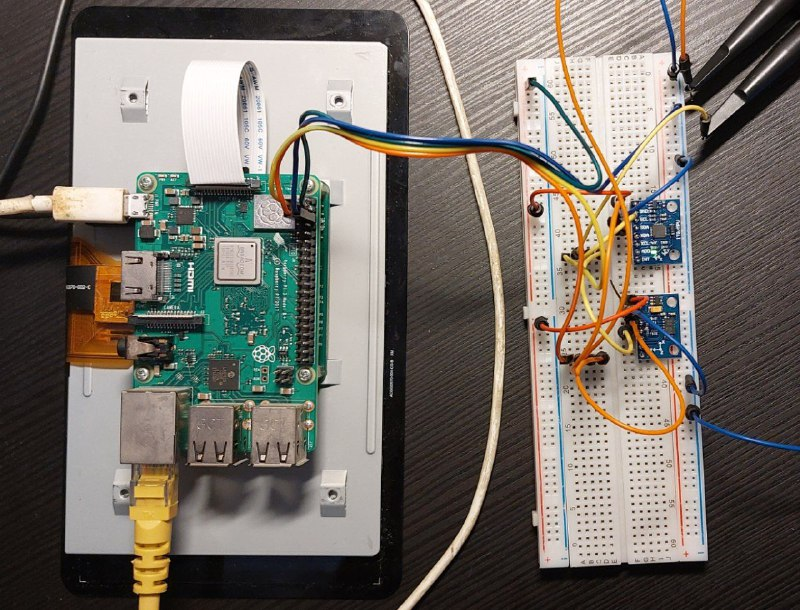
\includegraphics[width=0.6\textwidth]{figures/setup.jpeg}
\caption{Assembled HW setup}
\label{fig:setup}
\end{figure}

The MPU6050 was controled through the mpu6050 python3 library \cite{mpu_repo}. For the LSM3030DLHC board, there are two libraries (one for accelerometer \cite{acc_repo}, and one for magnetometer \cite{magn_repo}) ase the sensor appear on the $I^2C$ as two sepparate devices.

After some testing, it was observed that the magnetometer readings were very poor, probably because of presence of ferromagnetic materials (e.g. the breadboard). As a reasonably way to calibrate the magnetometer was not found after some research, the sensor has been dropped, and only the MPU6050 is used. Because of that, we can only measure pitch and roll. Yaw is not measurable.

The original goal was to implement the Kalman Filter directly on the RPi using python library numpy. But finally it was implemented with Octave/MATLAB computing the filter offline after the sensor data is recorded and transmitted to a computer with Octave/MATLAB.

The data is simply recorded in csv format. One row per each measure, and the columns feature the time stamp in seconds, the accelerometer measurement for the three axes (in $m/s^2$) and the gyroscope measurement for the three axes (in $\degree / s$).